%!TEX root = ../thesis.tex
\chapter{Introduction}
\label{ch:introduction}

%\epigraph{``As buds give rise by growth to fresh buds, and these, if vigorous, branch out and overtop on all sides many a feebler branch, so by generation I believe it has been with the great Tree of Life, which fills with its dead and broken branches the crust of the earth, and covers the surface with its ever-branching and beautiful ramifications.''}{Charles Darwin, 1872}

Darwin's \emph{On the Origin of Species} contains a single figure, depicting the ancestry of species as a branching genealogical tree \cite{Darwin:1859uh} (see Figure \ref{fig:darwin_origin}).
Since then, the tree structure has been the dominant framework to understand, visualize, and communicate discoveries about evolution.
Indeed, a primary focus of evolutionary biology has been to expand the \emph{universal tree of life}, the set of evolutionary relationships among all extant and extinct organisms on Earth \cite{Bowler:2003uz}.
Traditionally, this was the realm of phenotype-derived taxonomies.
With the advent of molecular sequene data and computational approaches for tree-inference, molecular phylogenetics has become the standard tool for inferring evolutionary relationships.
However, a tree is accurate only if the Darwinian model of descent via reproduction with modification is the sole process driving evolution.
It has long been recognized that there exist alterative evolutionary processes that can allow organisms to exchange genetic material through means beyond reproduction \cite{Arnold:2007vq}.
Notable examples include horizontal gene transfer in bacteria, species hybridization in plants, and meiotic recombination in eukaryotes.
Collectively, these processes are known as \emph{reticulate evolution}.
These stand in contast to descent with modification, an example of \emph{clonal evolution}.
\footnote{Clonal and reticulate evolution are also known by the terms \emph{vertical} and \emph{horizontal} evolution, respectively.}
Increasing genomic data, powered by new high-throughput sequencing technologies, has shown that these reticulate processes are more prevalent than originally expected.
For some, this has called into question the tree of life hypothesis as an organizing principle and prompted the search for new ways of representing evolutionary relationships \cite{Doolittle:1999,OMalley:2011tu}.

This thesis presents a new approach to quantifying and representing reticulate evolutionary processes using recently developed ideas from algebraic and computational topology.
The methods we employ fall under the collective heading of \emph{topological data analysis} (henceforth TDA), a new branch of applied topology concerned with inferring structure in high-dimensional data sets.
The thesis consists of three aims: (1) introduce the methods of TDA and their application to biological data, (2) develop approaches tailored to the unique problems and assumptions inherent in genomic data, and (3) apply these approaches to a wide range of biological datasets in which reticulate processes play an important role.

In the following brief introduction, we survey salient aspects of molecular evolution, the tree paradigm, and the challenges posed by reticulate processes.
We then introduce the idea of representing evolution as a topological space and give a flavor of the results to be discussed.

\begin{figure}
\centering
\includegraphics[width=.5\columnwidth]{./fig/introduction/Darwin_divergence.jpg}
\caption[Charles Darwin's Evolutionary Tree]{The only figure in Darwin's \emph{On the Origin of Species}. Darwin argued for descent with modification and natural selection as the driving processes underscoring evolution. In this figure, Darwin sketched his idea for how diverging species would result in a tree structure. Reproduced from \cite{Darwin:1859uh}.}
\label{fig:darwin_origin}
\end{figure}

\section{Molecular Evolution and the Tree Paradigm}

The combination of Darwin's theory of natural selection with Mendelian genetics led to the \emph{modern evolutionary synthesis}, outlined in the first half of the twentieth century in pioneering works by Ronald Fisher, Sewall Wright, JBS Haldane, and others.
\footnote{See \cite{Huxley:1942} and \cite{Gould:2002ts} for historical detail.}
The modern synthesis was based largely on an analysis of distributions of allele frequencies in distinct populations, the purview of classical population genetics.
The field was placed on a molecular foundation with Watson and Crick's discovery of the DNA double-helix in 1953 \cite{Watson:1953wm}.
These developments led to the establishment of \emph{molecular evolution}, the analysis of how processes such as mutation, drift, and recombination act to induce changes in populations and species.

The information underlying an organism's form and function is encoded in its genome, the complete sequence of DNA contained in each cell.
The genome can be represented as a string of nucleotides, indexed by position.
Embedded within the genome are regions defining the genes which code for functional proteins, as well as non-coding regions which have as-yet unknown function.
\footnote{In humans, only 1.5\% of the genome is protein-coding, the rest largely non-functional. \cite{Lander:2001hk}. Up to 5-8\% of the human genome is believed to consist of endogeneous retroviruses, dead viruses which have integrated their genome into the human genome.}
When an organism reproduces, either sexually or asexually, a complete copy of the genomic information is passed to the offspring.
Because the molecular mechanisms that control this copying are not exact, errors in replication are introduced.
These errors can take the form of single point mutations (or single nucleotide polymorphisms, SNPs) or small insertions and deletions of a few nucleotides (indels).
\footnote{Mutation rates vary across species. In humans, $10^{-8}$ per site per generation. In single cell bacteria, $10^{-10}$ per site per generation.}
Under the neutral theory of evolution, the majority of these errors will have very little impact, either positive or negative, on the descendant organism.
A small fraction of mutations will result in an appreciable fitness differential compared to other organisms, and it is on these organisms that natural selection will act.

While molecular biology has largely focused on the biochemical and biophysical mechanisms underlying these processes, \emph{molecular phylogenetics} has focused on the comparative analysis of macromolecular sequences to infer genealogical and evolutionary relationships.
Molecular phylogenetics began with Emile Zuckerkandl and Linus Pauling's recognition in the early 1960's that the information encoded in a set of molecular sequences could itself be used as a document of evolutionary history \cite{Zuckerkandl:1962,Zuckerkandl:1965wi}.
It became apparent that given two sequenced organisms, counting the differences between their respective sequences could be used as a quantitative measure of the amount of evolutionary divergence between the two.
If one has a larger set of sequenced organisms, computing the complete set of pairwise distances gives a \emph{distance matrix} for the organisms.
From the distance matrix, one attempts to associate a tree to the data such that pairwise distances along the tree are close to the pairwise sequence distances.
Walter Fitch and Emanuel Margolish helped popularized this approach by constructing a weighted least squares approach to fitting phlyogenetic trees from distance matrices \cite{Fitch:1967we}.
Since that time, the development of numerical approaches for inferring evolutionary relationships has evolved into a mature discipline and the use of molecular sequence data to infer phylogeny has become a standard practice across a wide range of biology and ecology.
While other approaches to tree inference have been developed, including parsimony, quartet analysis, and Bayesian methods, we will focus on distance matrix methods because of their close connection with the topological ideas we employ later.

% NEUTRAL THEORY: Not necessary to include?
% Two historical results, one from molecular evolution and one from molecular phylogenetics, are worth mentioning.
% First, Motoo Kimura's neutral theory of evolution, first detailed in 1968 \cite{Kimura:1968vw} (see \cite{Kimura:1984} for a comprehensive survey).
% The neutral theory holds that observed genetic diversity is largely a result of genetic drift.
% At the time the neutral theory was proposed, most biologists assumed that natural selection was the driving force behind genetic diversity.
% Kimura argued that at the molecular level, the vast majority of mutations are selectively neutral, that is they confer no fitness advantage to the individual organism.
% With increased sequencing of organisms and populations, tests for selection based on the neutral theory have been developed.

One important early result from molecular phylogenetics was Carl Woese's organization of bacteria, eukarya, and archaea into the three domains of life \cite{Woese:1977vd}.
Prior to Woese, there were two recognized domains of life: prokaryotes, single-celled organisms lacking a nucleus, and eukaryotes, multi-celled organisms with an enveloped nucleus.
Using 16S subunit ribosomal RNA sequencing, Woese discovered that the prokaryotic domain actually split into two evolutionarily distinct groups.
One of these, which he termed \emph{archaebacteria} was more closely related to eukaryotes than were there the rest of the prokaryotes.
This led to the three-domain system of life (see Figure \ref{fig:woese_tree}).

\begin{figure}
\centering
\includegraphics[width=.7\columnwidth]{./fig/introduction/woese_tree.png}
\caption[Carl Woese's Three Kingdom Tree of Life]{Carl Woese's three kingdom tree of life. Using 16S subunit ribosomal RNA, Carl Woese identified archaea as a distinct phylogenetic kingdom. Previously, based on morphological similarity (specifically, unicellular and lacking a nucleus), archaea had been grouped with bacteria. This result was an early success for molecular phylogenetics and the use of conserved gene segments for molecular classification. Figure adapted from \cite{Woese:1990uc}.}
\label{fig:woese_tree}
\end{figure}

This work had several important consequences.
First, it established the use of molecular data to inform about large-scale patterns of evolutionary history.
Using only morphological data had led to an inconsistent classification of archaea.
Second, it positioned 16S rRNA profiling as the primary source of data for use in comparative genomics.
The use of this genomic region was justified on the basis of being one of the few universal gene segments that is conserved across all species.
Constructing a universal tree is predicated on there being orthologous genes, shared genes related through speciation events, that can provide a common foundation for comparative study.
Finally, it solidified the tree paradigm as an organizing principle for relating extant species.
Even though reticulate processes had been known since the nineteenth century, the idea that evolutionary relationships should be described by a bifurcating tree had been paramount since Darwin. 
Reticulate processes were either ignored completely, or expected to occur at such low frequencies that they need not be considered.

\section{Reticulate Processes and the Universal Tree}

Despite the significant impact Woese's observation had, there remains a subtle difficulty, which Woese himself would come to contemplate in later work.
Woese's phylogeny was based on only 1,500 nucleotides in the ribosomal RNA, less than 1\% of the length of a typical bacterial genome (see \cite{Dagan:2006up}).
Even more striking, this accounts for less than 0.00005\% of the human genome.
While recent work has developed approaches for constructing reference trees from larger gene sets \cite{Ciccarelli:2006gw}, the fact remains that the vast majority of genomic information is \emph{not} incorporated into the tree.

The reason for this situation is twofold.
First, not all genes are shared universally across all species.
In constructing a phylogenetic tree using sequence data, only 
Second, even among universal genes, the presence of reticulate evolutionary processes will confound systematic analysis.

The model of a bifurcating tree is only consistent if.
When organisms exchange genetic material by means other than direct reproduction, ancestral relationships will be

If one were to use a different genomic region to construct a tree of species, a different tree topology would be generated.

Horizontal exchange occurs when a donor bacteria transmits foreign DNA into a genetically distinct bacteria strain.
Three mechanisms of horizontal transfer are identified, depending on the route by which foreign DNA is acquired \cite{Ochman:2000dr}.
Foreign DNA can be acquired via uptake from an external environment (transformation), via viral-mediated processes (transduction), or via direct cell-to-cell contact between bacterial strains (conjugation).

% HGT+Species concepts. Woese+Goldenfeld.
%\kje{(Expand more of the Doolittle story and the tree paradigm. Species concepts, etc..)}

Incompatibilities in the tree paradigm now appear as the rule, not the exception, demonstrating the need for new representations of evolutionary relationships \autocite{Doolittle:1999,Doolittle:2006}.
Many have argued that, in light of genomic evidence for the prevalence of reticulate processes, the very notion of a universal tree of life must be discarded.
One wonders if the information deduced from small genomic sections can be extrapolated to other regions, as different gene sequences can yield vastly different tree topologies.
\kje{[cite Doolittle, Koonin]}.
These and other similar situations, call for new methods of characterizing evolutionary relationships.

Finally, reticulate evolutionary processes are of more than just theoretical concern:
In HIV, frequent homologous recombination confounds our understanding of the epidemic's early and present history \cite{Burke:1997ep}.
In influenza, segmental gene reassortments lead to antigenic novelty and the emergenence of epidemics \cite{Nelson:2007bc}.
In several pathogenic bacteria, including \emph{E. coli} and \emph{S. aureus}, horizontal gene transfer has been responsibile for the spread of antibiotic resistance genes \cite{Ochman:2000dr,Alekshun:2007bq}.

\begin{figure}
\centering
\includegraphics[width=.8\columnwidth]{./fig/introduction/doolittle_tree.png}
\caption[Ford Doolittle's Reticulate Tree of Life]{W Ford Doolittle's representation of the universal tree of life with reticulate evolution. While the three domains of life are still recognizable, patterns of divergence no longer follow a strictly treelike model. (From \emph{Science}, vol. 284, issue 5423, page 2127. Reprinted with permission from AAAS.)}
\label{fig:doolittle_tree}
\end{figure}

\section{Evolution as a Topological Space}

We propose the use of new computational techniques, borrowed from the field of applied topology, to capture and represent complex patterns of reticulate evolution.

Topology as a mathematical field is concerned with properties of spaces that are invariant under continuous deformation.
Such properties can include, for example, connectedness and the presence of holes.
Objects are considered topologically equivalent if they can be deformed into one another without introducing cuts or tears.
As a paradigmatic example, consider the coffee mug and the donut (Figure~\ref{intro:fig:coffeemug_to_donut}).
While seemingly different, it is not difficult to see that both objects consist of a single connected component that is wrapped around a single hole, and can be freely deformed into one another.
Topologically, the two objects are equivalent.\footnote{The two objects are topologically equivalent to a solid torus, which can be represented as $D^2\times S^1$, a solid two-dimensional disk wrapping around a circle.}

\begin{figure}[t]
\centering
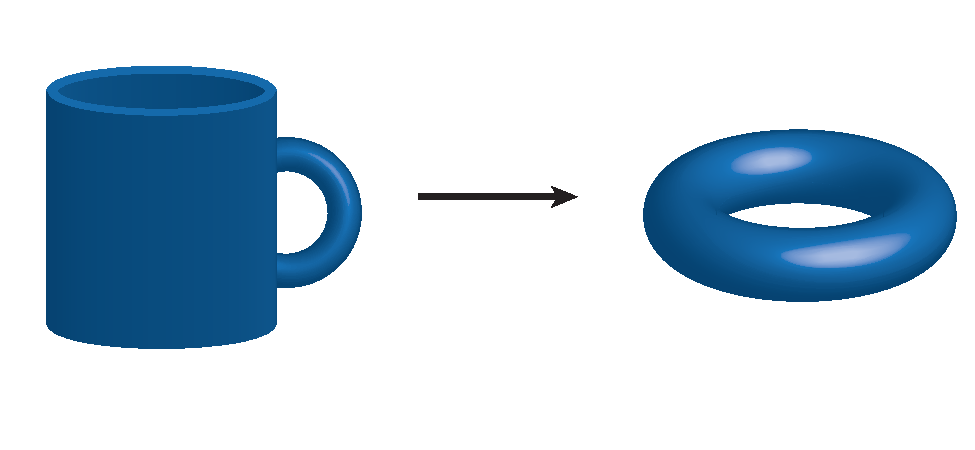
\includegraphics[width=\columnwidth]{./fig/introduction/coffeemug_to_donut.pdf}
\caption[The coffee mug and the donut]{The paradigmatic topology example. The coffee mug can be continuously deformed into the donut and are therefore topologically equivalent. Both exhibit the topology of a solid torus ($D^2\times S^1$).}
\label{intro:fig:coffeemug_to_donut}
\end{figure}

Algebraic topology quantifies our intuitive notions of shape by associating algebraic structures to different invariants.
For our purposes, the most relevant invariants will be the \emph{Betti numbers}.
We give a more complete characterization of Betti numbers in Chapter~\ref{ch:background}, but the intuition is as follows.
First, we can think of $b_0$ as representing the number of connected components, or clusters, in our space.
Next, we can think of $b_1$ as representing the number of loops in our space.
Equivalently, this is the number of cuts needed to transform the space into something contractible to a point.
Higher Betti numbers, $b_n$ for $n>1$ will correspond to higher dimensional holes.
In our coffee mug example, because both objects have the same Betti numbers ($b_0=1$, $b_1=1$, and $b_n=0$ for $n>1$), they can be considered topologically equivalent.
Our goal in this work will be to adopt a similar perspective as this example and characterize evolutionary spaces as topological spaces using their Betti numbers.

To give the very simplest example, consider Figure~\ref{intro:fig:simple_tree_example}.
On the left we have a simple rooted three leaf evolutionary topology.
There is a single connected component that is trivially contractible, giving $b_0=1$ and $b_1=0$.
By trivially contractible we mean it can be deformed into a point, a property which will hold for all tree topologies.
On the right, we have a reticulate topology again involving three leaves.
We can envision the center leaf as being a reticulate offspring of parents ancestral to the left and right leaves.
That is, the center leaf carries some genetic material from both the left and right branches.
Accounting for this reticulation generates a single loop, giving $b_0=1$ and $b_1=1$.
The object is no longer treelike and is characterized by a nontrivial topology.
The Betti numbers capture the essential difference in the two evolutionary histories.

Consider again Darwin's branching phylogeny (Figure~\ref{fig:darwin_origin}) and Doolittle's modified tree accounting for reticulate evolution (Figure~\ref{fig:doolittle_tree}).
The two objects can be imagined to be representations of two different topological spaces.
Darwin's branching phylogeny is a tree and hence trivially contractible ($b_n=0$ for $n>0$).
In contrast, Doolittle's construction has a much more complex topology, with loops being formed at points where reticulate events have occurred.
The object will have nonvanishing Betti numbers, which will be associated with the amount of reticulation.
The remainder of this thesis focuses on expanding this idea and applying it to real data sets with the goal of measuring the prevalence and scale of reticulate evolutionary events.
Our aim will be to characterize reticulate exchanges of genetic material by the parental sequences involved in the exchange, by the amount and identity of material exchanged (i.e., the genes or loci involved), and the frequency with which similar exchanges occur.
Several important questions will be dealt with, such as how to construct topological spaces from finite samples, how to make comparisons among gene sets, and how to make statistical statements about reticulate events.
We will address these questions, and in doing so develop new techniques to construct and extract topological and statistical information from evolutionary data.
In doing so, we provide a fuller understanding of evolutionary relationships than allowed by current phylogenetic methods.

\begin{figure}
\centering
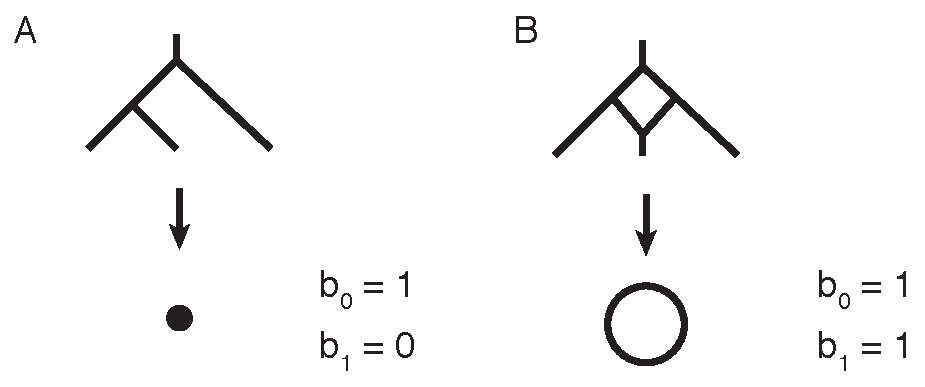
\includegraphics[width=.8\columnwidth]{./fig/introduction/simple_tree_example.pdf}
\caption[Treelike and reticulate phylogenies]{(A) A simple treelike phylogeny is contractible to a point. (B) A reticulate phylogeny that is equivalent to a circle and not contractible without a cut. The two spaces are not topologically equivalent and can be distinguished by their Betti numbers.}
\label{intro:fig:simple_tree_example}
\end{figure}

% (a good sentence but move to background)
% Techniques such as phylogenetic networks and ancestral recombination graphs have been developed to describe reticulate evolution, but they have had only limited success due to difficulties of biological interpretation and computational infeasibility in all but the smallest datasets.

% Linkage-based techniques have succeeded in measuring rates of recombination in medium-sized datasets (<200 sequences), but they cannot reveal the scale of these exchanges (i.e., the genetic distance between parental sequences), and they have limited resolution in pinpointing where along a genome such exchanges have occurred.
% A new mathematical foundation is needed to move beyond these limitations.
% Genome evolution is an extremely rich subject [cite Genome Architecture book].

\section{Thesis Organization}

The remainder of this thesis is organized as follows.

In Chapter \ref{ch:background} we present background material on the topics discussed in this thesis.
This discussion is chiefly structured into two pieces: (1) background on phylogenetics and population genetics, and (2) background on the methods we use from TDA.

In Part \ref{part:theory}, we develop two complementary approaches for analyzing sequence data using TDA.
In Chapter \ref{ch:complex_construction}, we propose methods of constructing topological spaces that generalize standard constructions but are suite to the particular requirements of phylogenetic applications.
We draw on previous work in phylogenetic networks and use homology to provide a quantitative assessment of reticulate processes.
This work was published in \cite{Emmett:2015a}.
In Chapter \ref{ch:parametric_inference}, we develop methods for performing statistical inference using summary statistics computed using methods from TDA.
This is the first such use of TDA as a tool for performing parametric inference and should generalize to a wide range of application settings.
This work was published in \cite{Emmett:2014b}

In Part \ref{part:applications}, we apply our approach to several problems in evolution and genomics.
In Chapter \ref{ch:phage} we study bacteriophages.
In Chapter \ref{ch:influenza} we study influenza.
In Chapter \ref{ch:pathogens} we study pathogenic bacteria and use topological techniques to represent the spread of antibiotic resistance.
In Chapter \ref{ch:prokaryotes} we study prokaryotic evolution and species tree topologies.
In Chapter \ref{ch:human_recombination_rate} we use population data to measure human recombination rates and identify recombination hotspots.
We identify variation in recombination hotspots in different human populations.
In Chapter \ref{ch:human_chromatin_folding} we analyze Hi-C data to explore patterns of chromatin folding in the nucleus in both prokaryotic and human datasets.

Finally, in Chapter \ref{ch:conclusions} we summarize these results and present future research directions.